\chapter{Modelling}

\section{Motivation}
\begin{definitionbox}{System Model}
    \begin{center}
        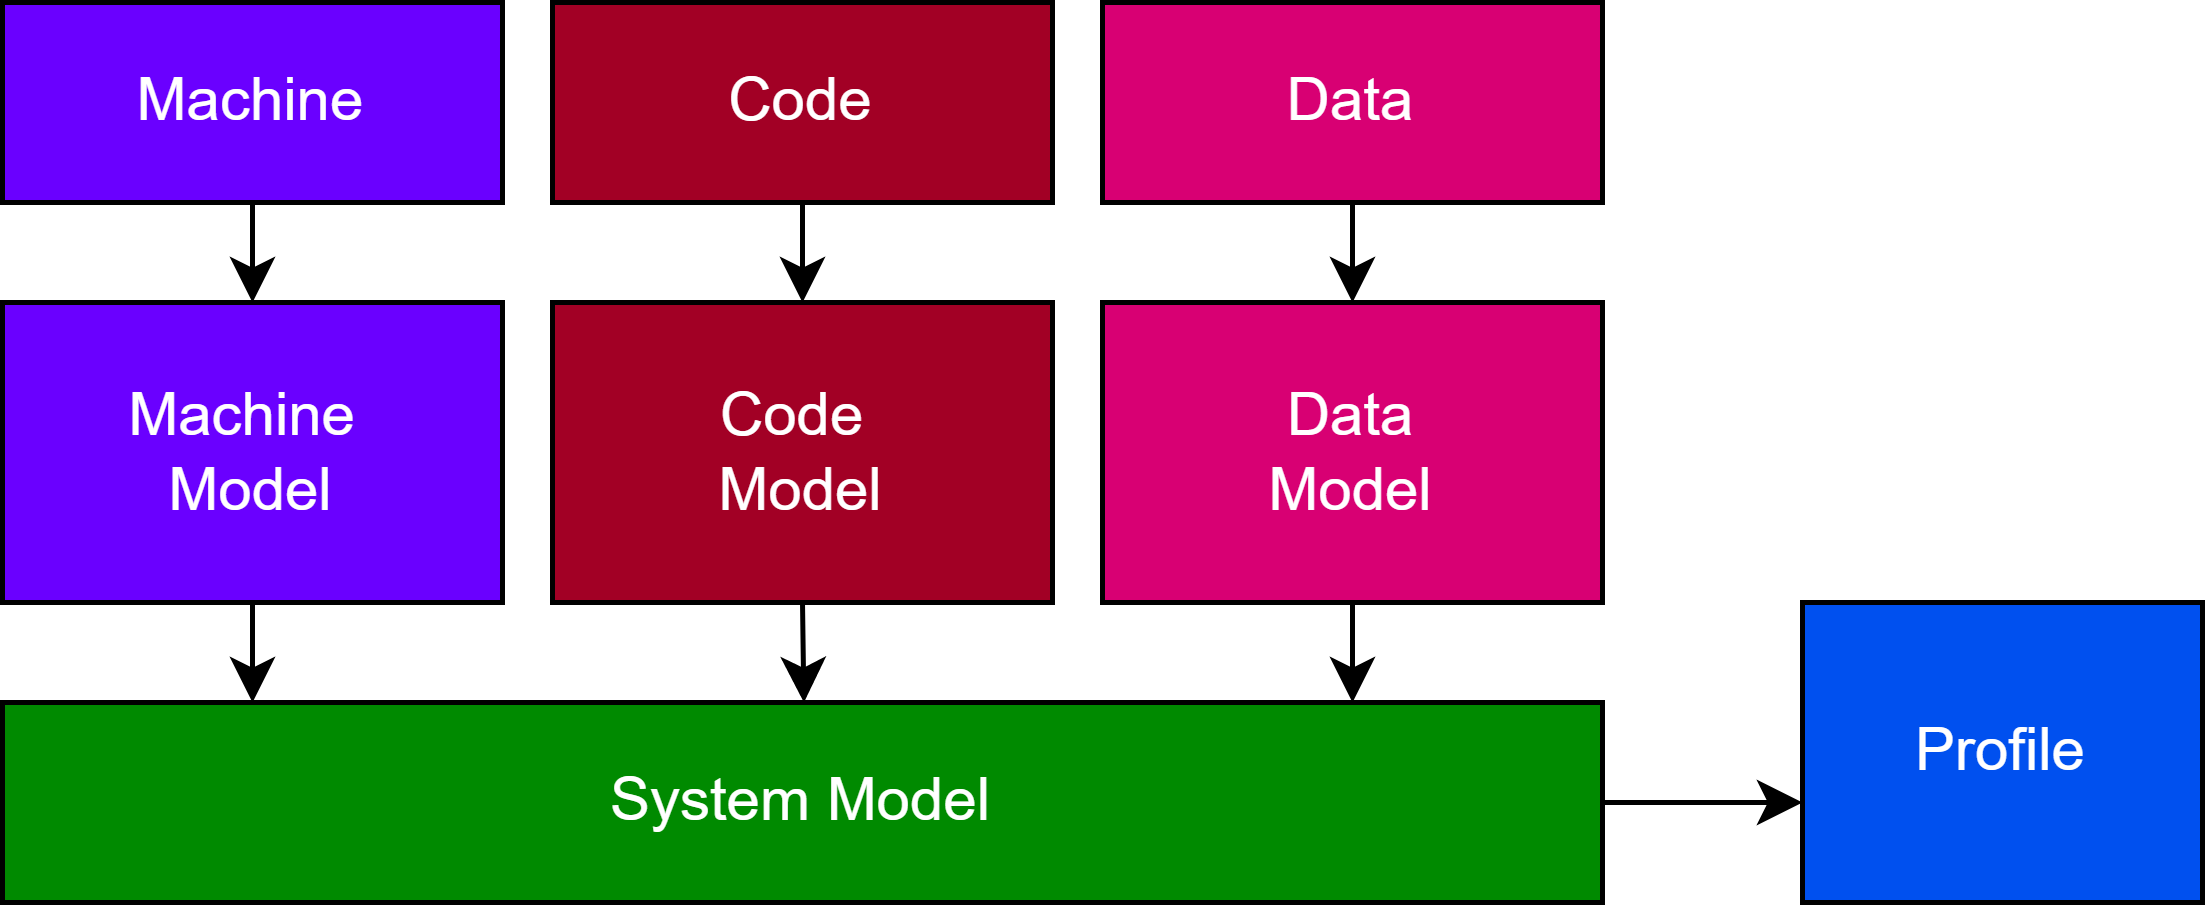
\includegraphics[width=.6\textwidth]{modelling/images/system_model.drawio.png}
    \end{center}
    A model used to characterise the performance of a system. Used to estimate performance without the overhead of running the system.
\end{definitionbox}

During this course we make several simplifying assumptions:
\begin{itemize}
    \item {\textbf{Input Data from a Known Distribution}
        \\ Typically uniform. We avoid complications form correlated inputs. 
    }
    \item {\textbf{No System Noise}
        Noise caused by the operating system  (scheduling, other processes actions) and other factors.
    }
    \item {\textbf{Single Threaded \& Deterministic Code}
        Modelling parallel systems requires considering contention and is an open area of research. 
    }
\end{itemize}

\section{Numerical Models}
\begin{definitionbox}{Numerical Model}
    Empirical measurement of the observed behaviour of the system.
    \begin{itemize}
        \item Describes actual system behaviour (is a measurement)
        \item Prediction limited $\to$ depends on the human interpretation of the data.
    \end{itemize}    
\end{definitionbox}

\begin{tabbox}{prosbox}
    \textbf{Easy To Create} & As long as the system is available to run benchmarks on. \\
    \textbf{True} & It is an empirical measurement of the actual system (or some component of it). \\
    \textbf{Easy to Interpret} & We can easily see how performance metrics vary with a given parameter. \\
\end{tabbox}
\begin{tabbox}[.7\textwidth]{consbox}
    \textbf{Poor Generalisation} & We cannot easily apply measurements to new values for parameters (mainly descriptive model / poor prediction) \\
    \textbf{Costly} & For a large number of parameters, high fidelity a large amount of data is required, and hence many runs of benchmarks. \\
    \textbf{Limited Prediction} & We can infer predictions from measurement, but it is difficult to extrapolate with confidence. \\
\end{tabbox}

\begin{definitionbox}{Microbenchmark}
    Small programs designed to test a specific portion of a system.
\end{definitionbox}


Numerical Models are constructed by:
\begin{enumerate}
    \item Data (performance metrics) gathered through \textit{microbenchmarks} on a range of parameter values.
    \item Data is analysed/interpreted.
\end{enumerate}

\section{Analytical Models}
\begin{definitionbox}{Analytical Model}
    A formalised relationship between system parameters and performance metrics.
    \begin{itemize}
        \item Hard to interpret (limited descriptive use)
        \item Evaluating the model (given parameters) predicts performance metrics
        \item A detailed understanding of the system is required
        \item Model must be validated using experimental data
    \end{itemize}
    Models can even be used inside the system itself. For example using an analytical model to determine which optimiser to use for a query plan 
\end{definitionbox}

\begin{sidenotebox}{Example Models}
    An example of a cost model for an R-Tree can be found in
    \href{https://ieeexplore.ieee.org/document/655810}{Cost models for join queries in spatial databases}.
    \\
    \\ The \href{https://dsl.cds.iisc.ac.in/projects/PICASSO/}{Picasso Database Query Optimizer Visualizer} another example of analytical models being used in the context of databases.
\end{sidenotebox}

\subsection{Empirical to Analytical}
We fit an analytical model via regression on data from a numerical model.

\subsubsection{Benchmark}
For example we could benchmark the memory system of a machine:
\inputminted{C}{modelling/code/access.c}

\subsubsection{System Parameters}
\begin{tabular}{l l}
    $B_0$ & Size of a General Purpose Register of the CPU \\
    $B_1$ & Size of a cache line of the Level 1 cache \\
    $B_2$ & Size of a cache line of the Level 2 cache \\
    $B_3$ & Size of a Memory Page \\
    $l_0$ & Access Latency of the Level 1 Cache \\
    $l_1$ & Access Latency of the Level 2 Cache \\
    $l_2$ & Access Latency of the main memory \\
    $l_3$ & Lookup time in the Page Table \\
    $C_0$ & Capacity of a General Purpose Register of the CPU \\
    $C_1$ & Capacity of the Level 1 Cache \\
    $C_2$ & Capacity of the Level 2 Cache \\
    $C_3$ & Number of Memory Pages in the TLB $\times$ Page size \\
\end{tabular}

\subsubsection{Model}
Given $s$ is the stride parameter in the characteristic equations:
\[T_{Mem} = \sum_{i = 0}^3 l_i \times \min\left(1, \cfrac{s}{B_i}\right) \ \text{ or we could model as } \ T_{Mem} = \begin{cases}
    l_0 & s < C_1 \\
    l_0 + l_1 & s < C_2 \\
    l_0 + l_1 + l_2 & s < C_3 \\
    l_0 + l_1 + l_2 + l_3 & otherwise \\
\end{cases}\]
We can compare the effects of altering system parameters on both models.

\subsubsection{Fitting}
Some parameters can be taken from documentation, others may be derived from experiment.
\\
\\ Ideally the model should automatically self-tune to set parameters. Automating the tuning process has several advantages:
\begin{itemize}
    \item Less work required by humans.
    \item Can adapt to changing conditions (e.g if cache size is artificially reduced by contention for shared cache my many threads)
    \item Can scale forward (if CPU is updated to newer generation, model can be re-tuned to fit changed system parameters)
\end{itemize}


\section{Memory Access Patterns}
\subsection{Memory Region}
\begin{center}
    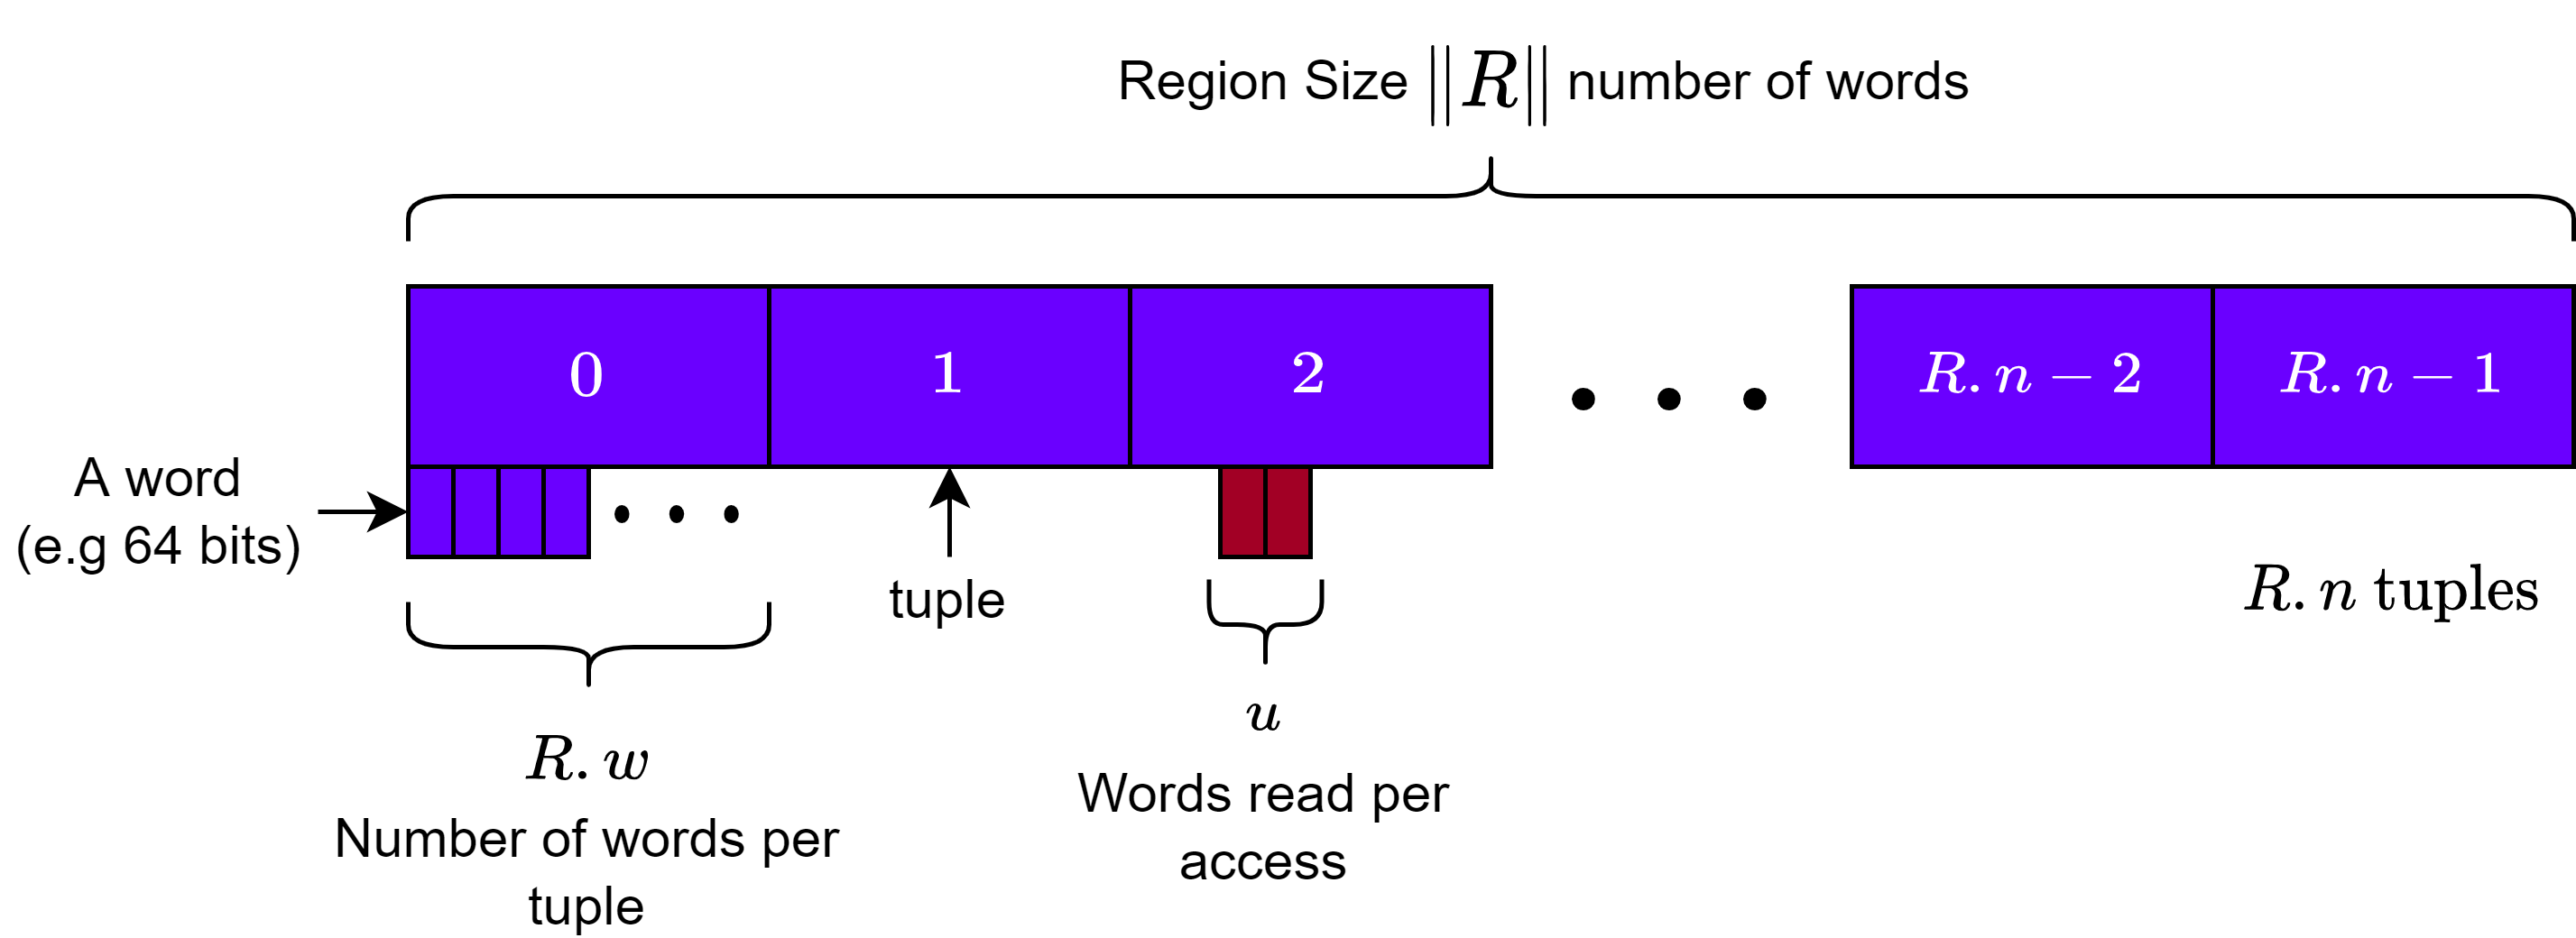
\includegraphics[width=.8\textwidth]{modelling/images/memory_region.drawio.png}
\end{center}
\begin{itemize}
    \item The number of words skipped over between each access is $R.w - u$
\end{itemize}

\subsection{Sequential}
\begin{center}
    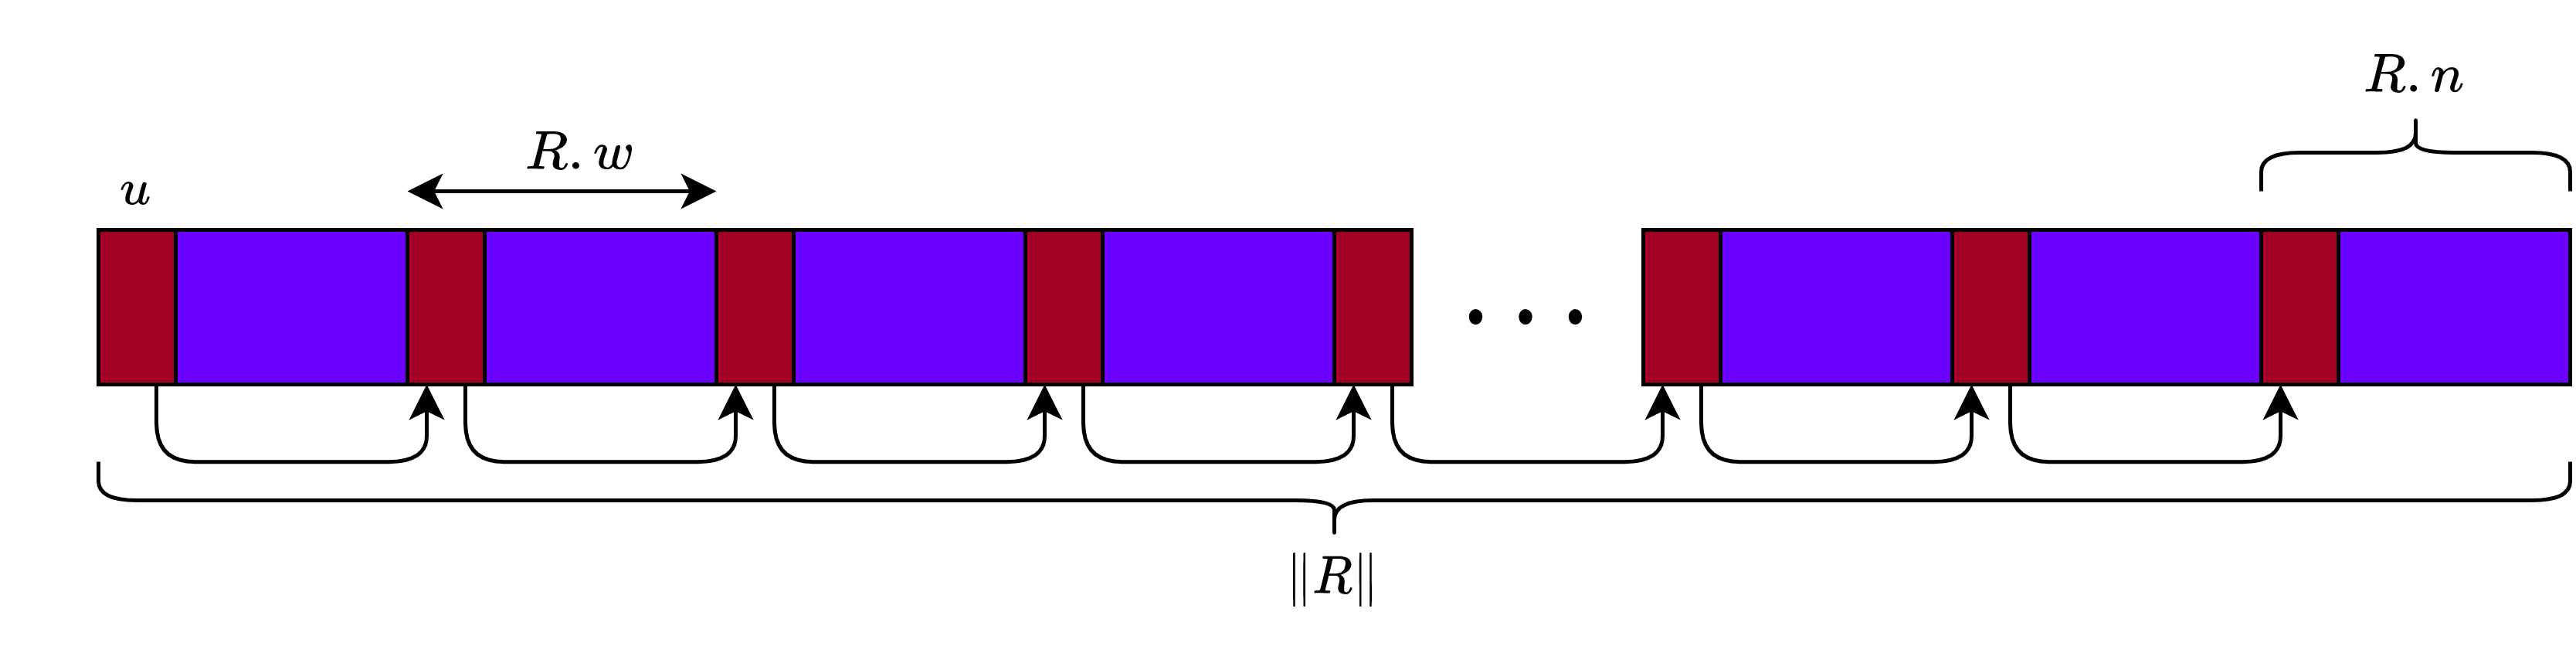
\includegraphics[width=.8\textwidth]{modelling/images/sequential_access_u_1.drawio.png}
\end{center}
Given some block size we can estimate the number of misses with a simple model.
\begin{itemize}
    \item Assume a cold start (no part of the region in cache already)
    \item Assume accesses are within blocks, not over boundaries (e.g if $u > 1$ and went over the edge of a cache line)
    \item $s\_trav$ means \textit{sequential traversal}
\end{itemize}
\[M_i^s(s\_trav) = \begin{cases}
    \cfrac{\| R \|}{B_i} & R.w - u < B_i \\
    R.n \times \left\lceil \cfrac{u}{B_i} \right\rceil & R.w - u \geq B_i \\
\end{cases}\]
\begin{center}
    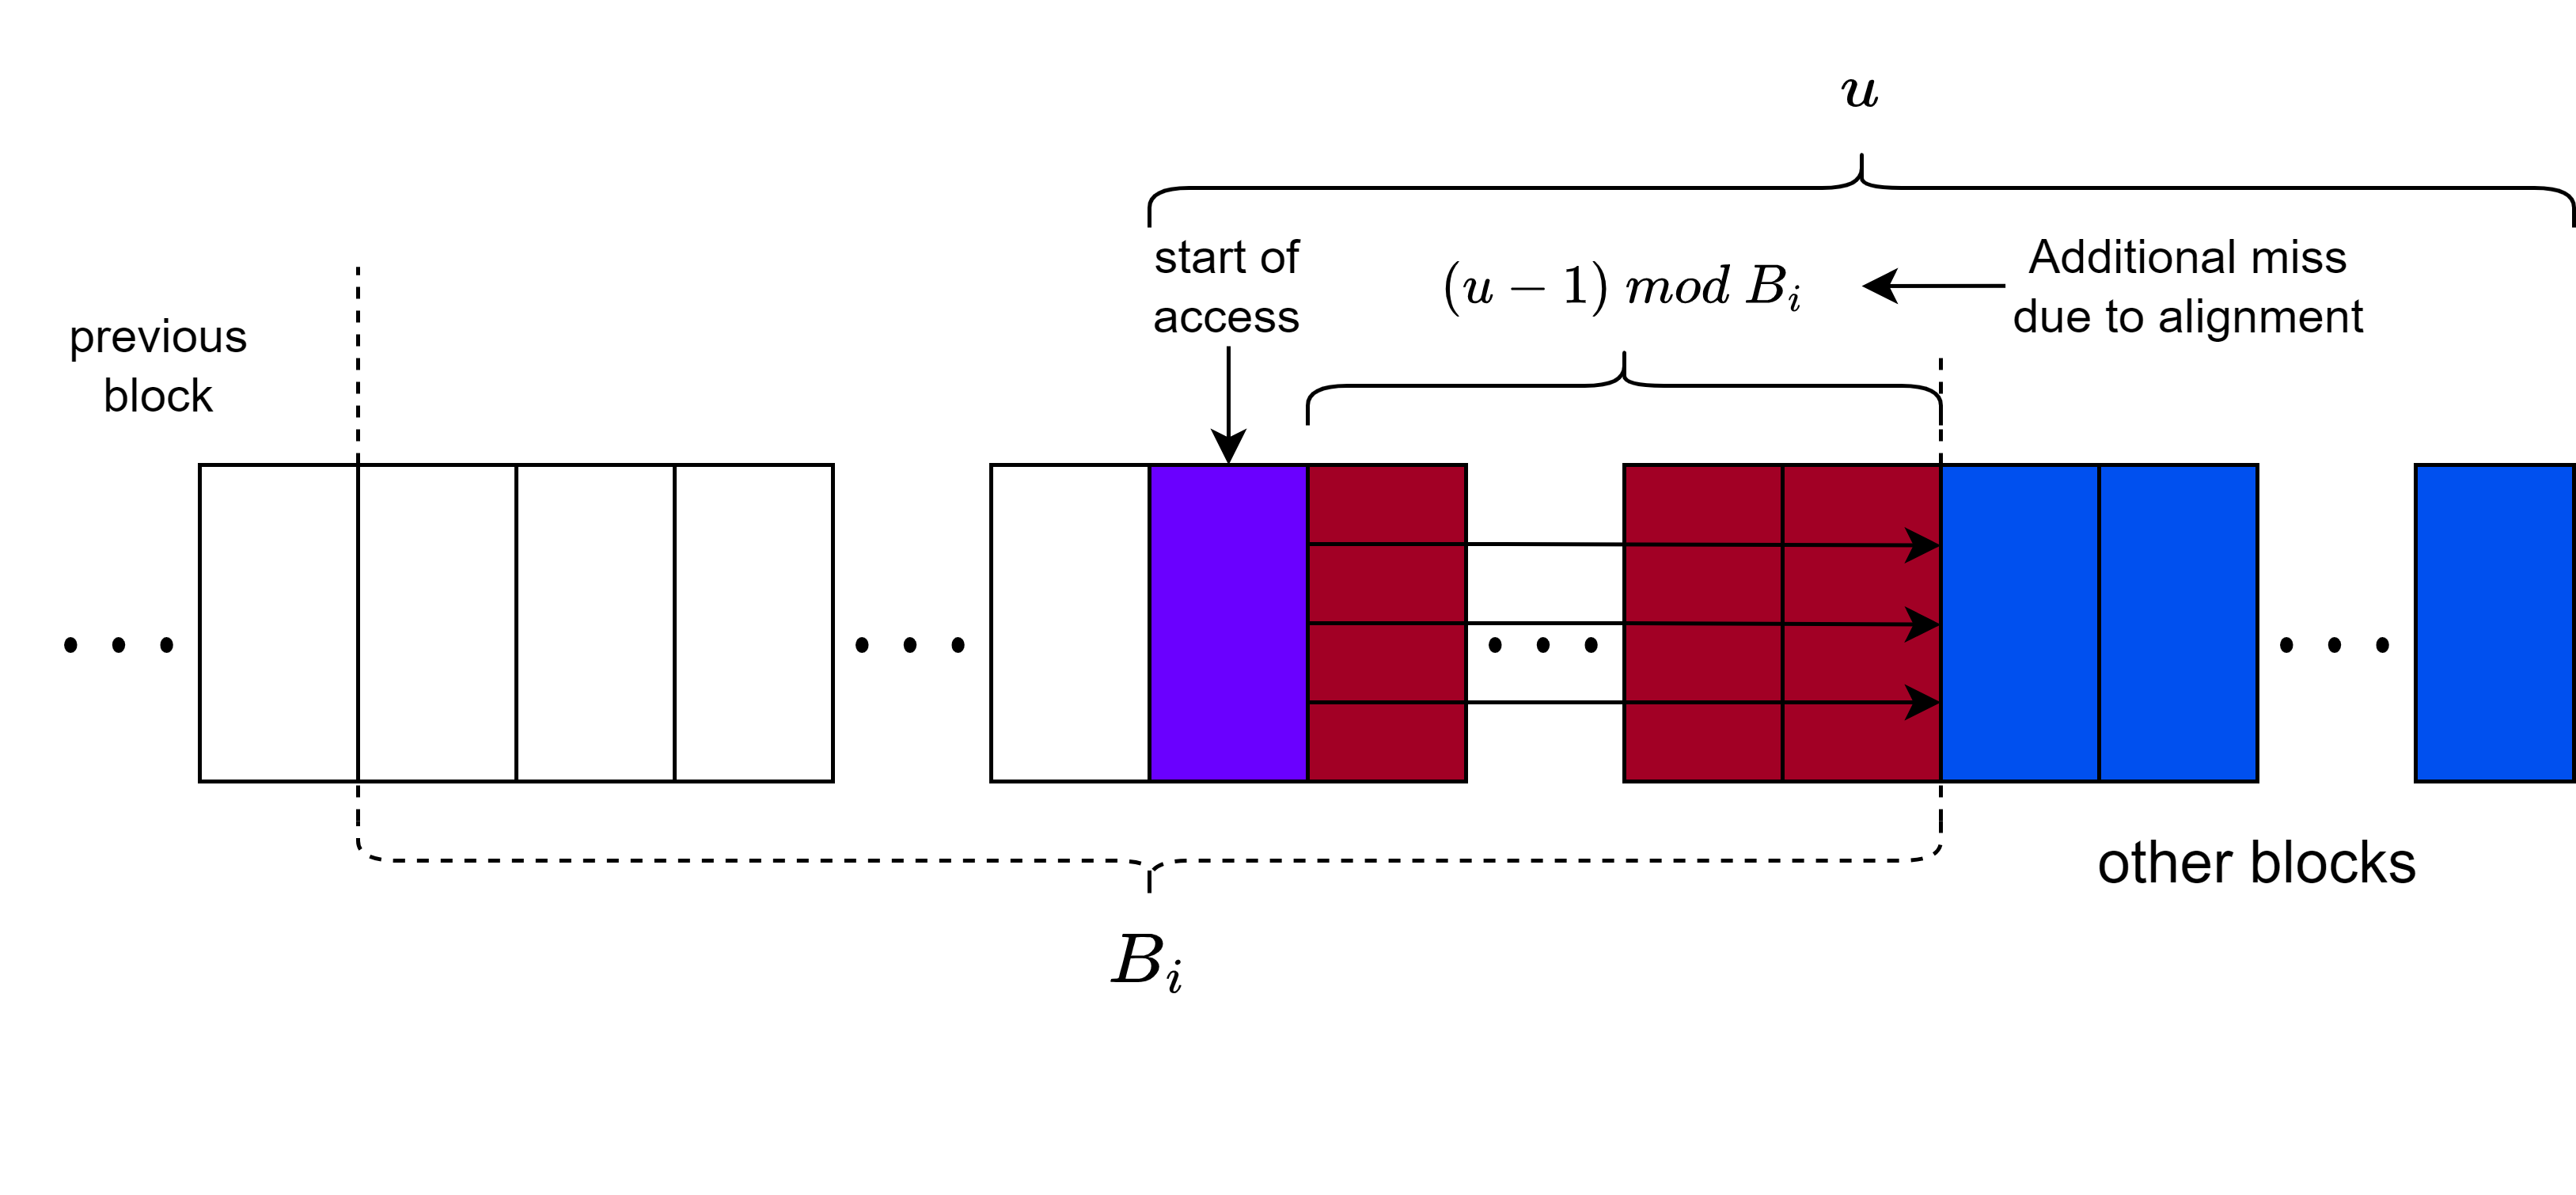
\includegraphics[width=.7\textwidth]{modelling/images/alignment_miss.drawio.png}
\end{center}
We may want to consider additional misses due to misalignment ($u$ stretching over two $B$s), in which case we much change the $R.w - u \geq B_i$ case to:
\[M_i^s(s\_trav) = R.n \times \left(\left\lceil \cfrac{u}{B_i} \right\rceil + \cfrac{(u-1) \mod B_i}{B_i} \right)\]

\subsection{Repetitive Random Access}
\[M_i^s(rr\_acc) = \text{undefined in lecture}\]
\begin{center}
    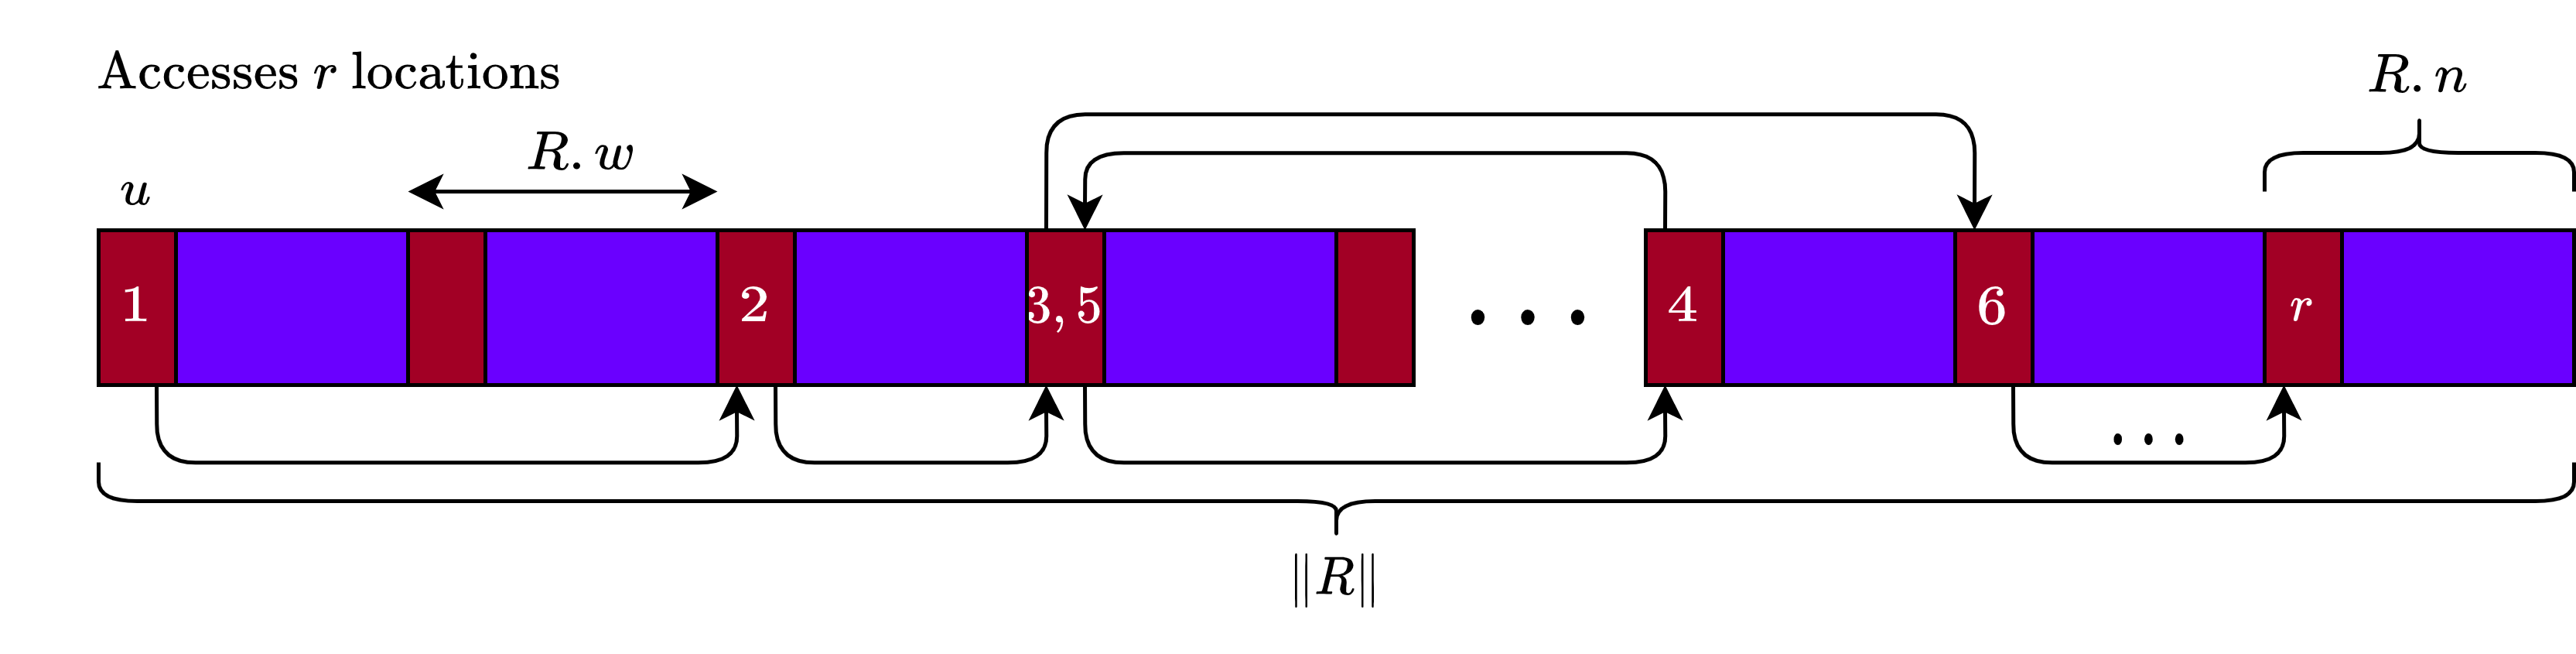
\includegraphics[width=.8\textwidth]{modelling/images/random_access.drawio.png}
\end{center}
Randomly access $r$ locations (can repeat accesses)

\subsection{Random Traversal}
\[M_i^s(r\_trav) = \text{undefined in lecture}\]
\begin{center}
    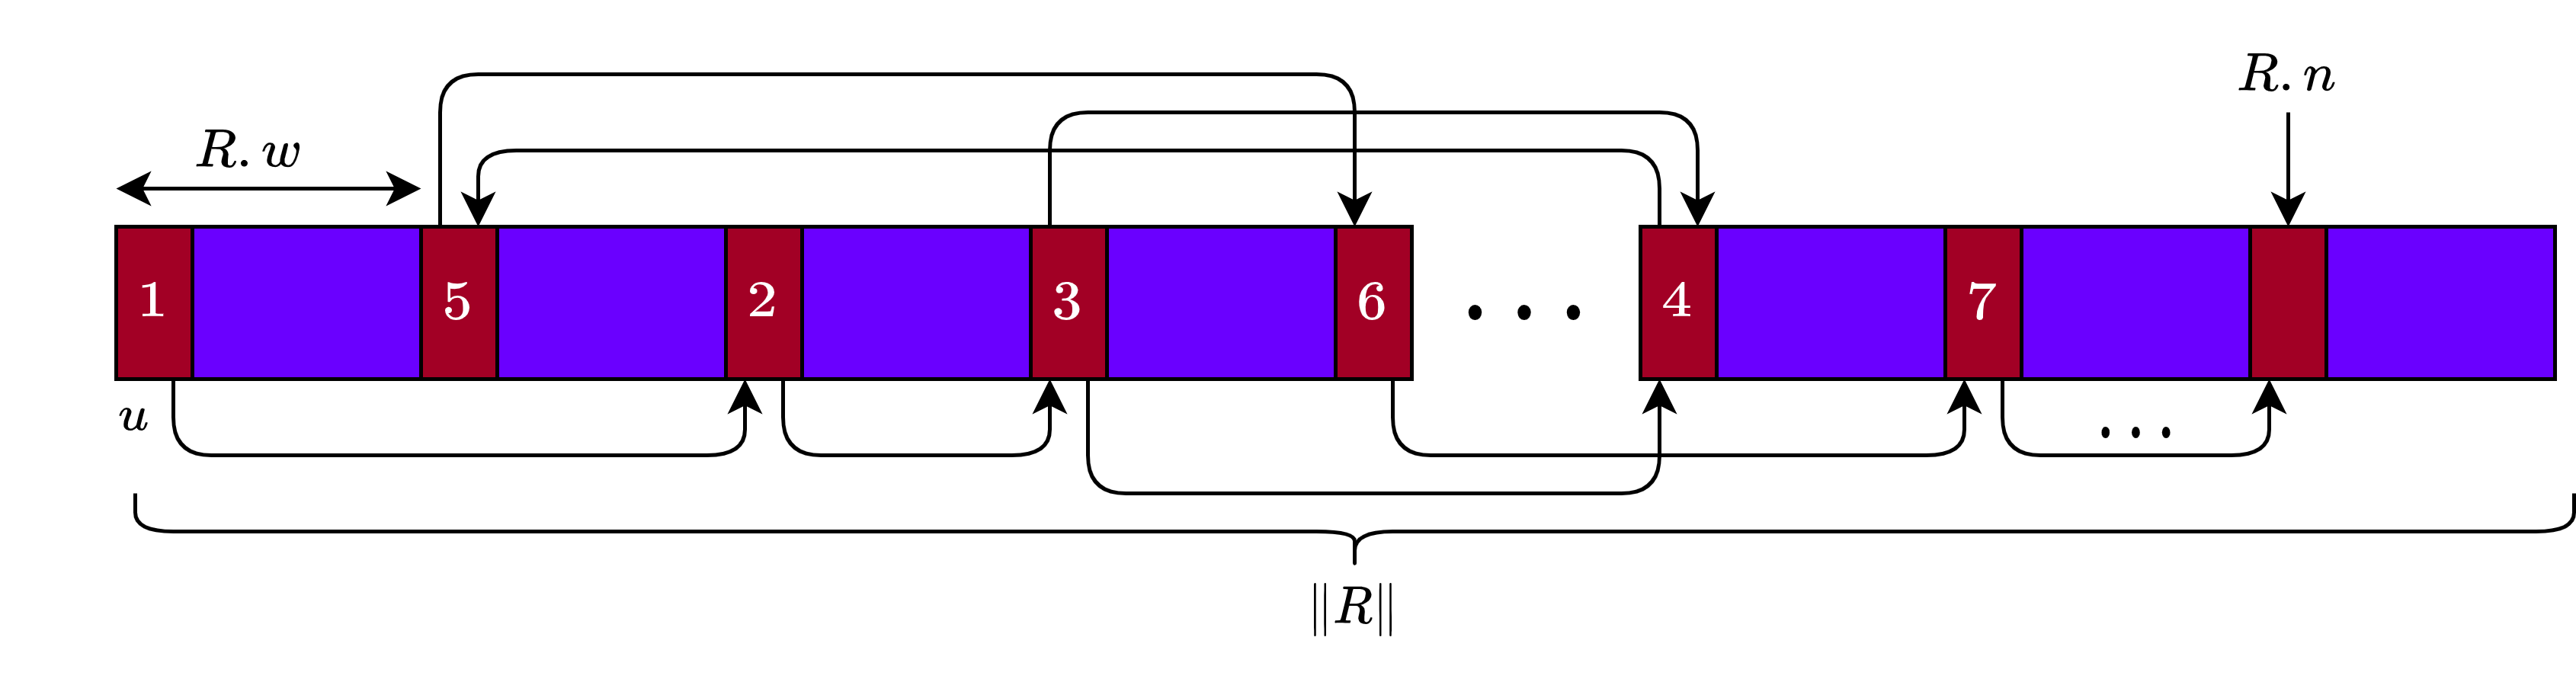
\includegraphics[width=.8\textwidth]{modelling/images/random_traversal.drawio.png}
\end{center}
Access all $R.n$ locations in some random order.

\subsection{Modelling Complex Patterns}
\begin{center}
    \begin{tabular}{l p{.8\textwidth}}
        $\mathcal{P}_1 \oplus \mathcal{P}_2$ & Sequential execution of patterns $\mathcal{P}_1$ then $\mathcal{P}_2$. \\
        $\mathcal{P}_1 \odot  \mathcal{P}_2$ & Concurrent execution (access patterns interleaved). \\
    \end{tabular}
\end{center}
We can hence combine access patterns.

\begin{examplebox}{Random Arrays}
    Create an access pattern description for the following program.
    List any other assumptions.
\begin{minted}{C}
#include <stdint.h>
#include <stddef.h>

extern int32_t input_data_1[i]; // uniform random data (used for index)
extern int32_t input_data_2[j]; // random data
extern size_t N;              // A large constant

void benchmark() {
    int32_t sum = 0;
    for (size_t i = 0; i < N; i++)
        sum += input_data_2[input_data_1[i]];
}
\end{minted}
    \tcblower
    We assume that $N = i$ and all entries of \mintinline{C}{input_data_1} $x$  are such that $0 \leq x \leq i$ (otherwise array accesses can be out of bounds)
    \[s\_trav(R.w = 1, u = 1, R.n = i) \odot rr\_acc (R.w = 1, u = 1, R.n = j, r = i)\]
\end{examplebox}

More complex access patterns can be modelled.
\[\underbrace{s\_trav(\dots) \odot r\_trav(\dots)}_{\text{Hash Join Build}} \oplus \left( \underbrace{\underset{\text{Read Input}}{s\_trav(\dots)} \odot \underset{\text{Access Hashtable}}{rr\_acc(\dots)} \odot \underset{\text{Write Output}}{s\_trav(\dots)}}_{\text{Hash Join Build}} \right)\]

\section{Modelling State}
Analytical models are stateless, but most systems have some kind of dynamic state that can influence behaviour and performance.
\\
\\ Stochastic models can be used to encode state (combine analytical models and dynamic state).
\begin{definitionbox}{Discrete Time Markov Chains (DTMC)}
    A stochastic model describing a sequence (discrete time steps) of possible states.
    \begin{center}
        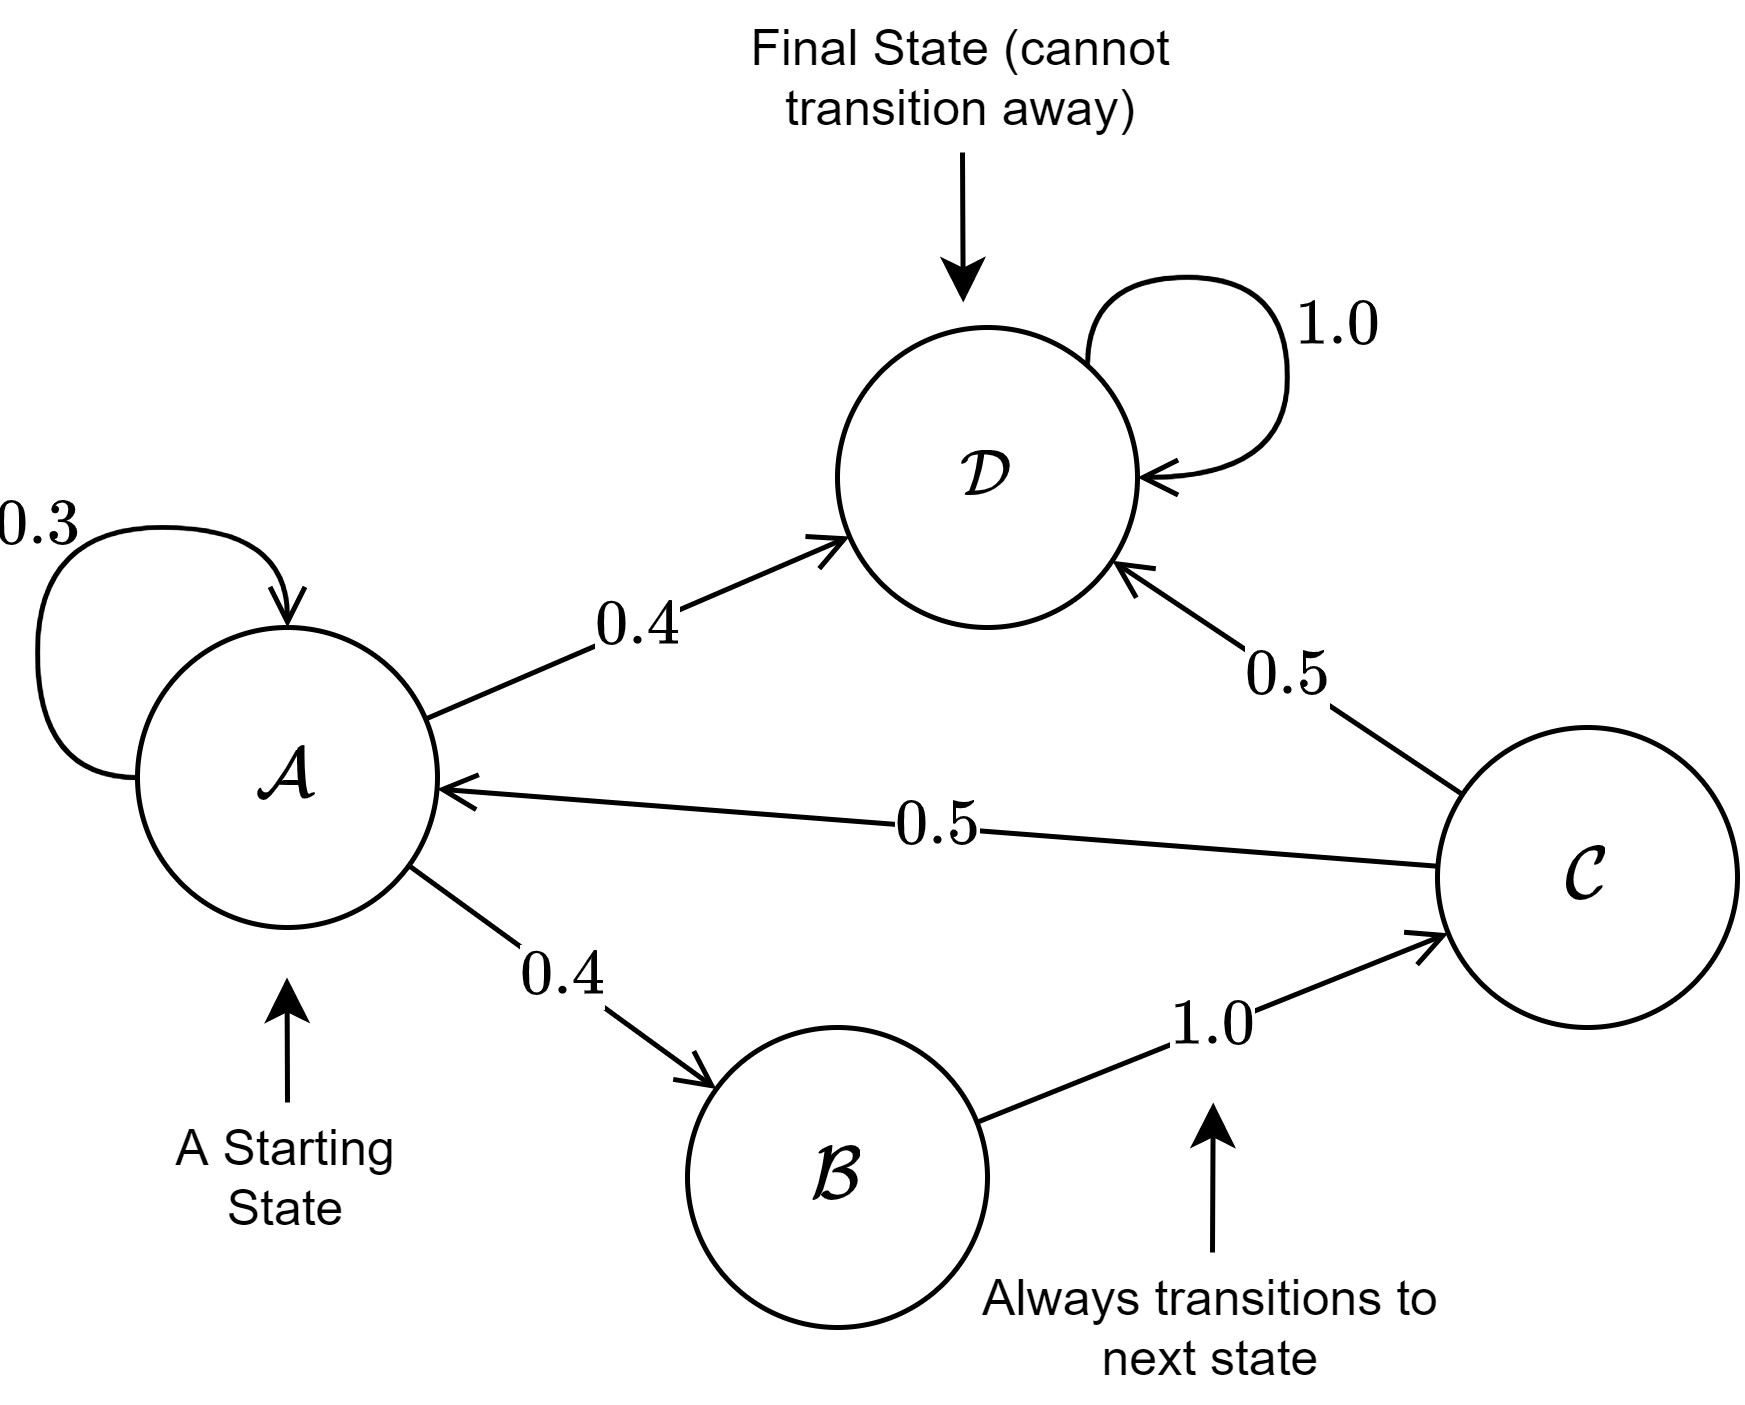
\includegraphics[width=.6\textwidth]{modelling/images/dtmc.drawio.png}
    \end{center}
    \begin{itemize}
        \item Much like a probabilistic finite state machine $\to$ the next state is only dependent on the previous (and random variables for transition) (called the \textit{markov property}).
        \item Transition probabilities out of a state must sum to $1$
        \item Can be represented as a matrix (directed graph represented as an adjacency matrix)
    \end{itemize}
\end{definitionbox}

\subsection{Simple Branch Direction Prediction}
Consider a simple conditional branch, to a known target (instruction). For example a basic loop:
\begin{minted}{C}
int N = 42;

void a() {
    int i = 0;
    while (i < N) {
        i++;
    }
}
\end{minted}
Compiled for x86 with \mintinline{bash}{-O1} (\href{https://godbolt.org/z/1xedvGbx9}{godbolt}) we get the following:
\begin{minted}{asm}
a:
    ; Load N to edx and determine if any loop iteration should run (N may be 0)
    mov     edx, DWORD PTR N[rip]
    test    edx, edx

    ; Start looping
    jle     .L1        ; [Conditional branch, known target]
    mov     eax, 0     ; int i = 0
.L3:
    add     eax, 1     ; i++
    cmp     eax, edx   ; Check that i < N by checking if i == N yet
    jne     .L3        ; [Conditional branch, known target]
.L1:
    ret                ; [Conditional branch, unknown target -> target prediction with RAS]
N:
    .long   42
\end{minted}

We will focus on the conditional branches with a known target (target prediction is more complex).
\begin{center}
    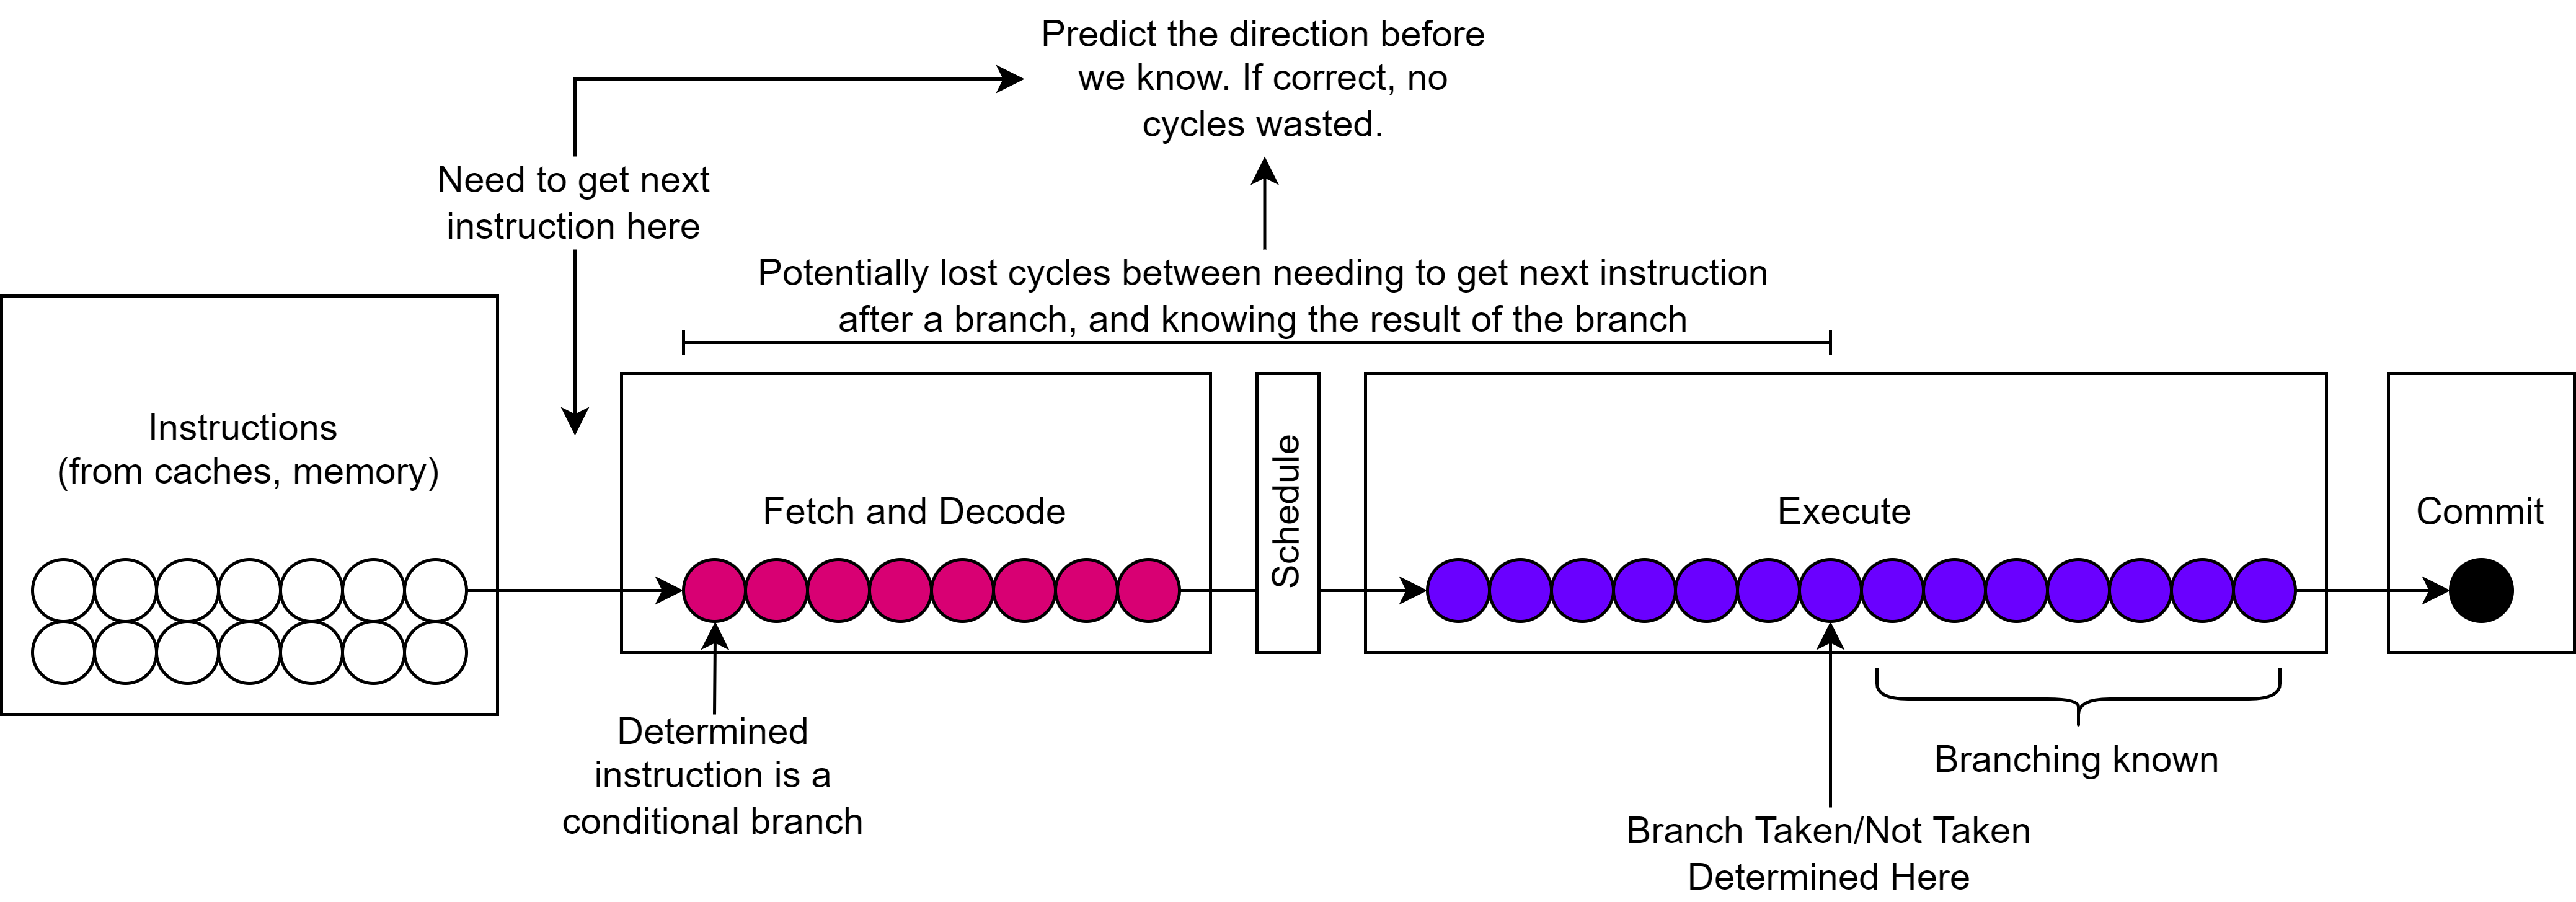
\includegraphics[width=.9\textwidth]{modelling/images/branch_direction_prediction_motivation.drawio.png}
\end{center}
There are several ways to reduce potential penalty from branch instructions:
\begin{itemize}
    \item Smaller frontend (reduce cycles between fetch and branch determination).
    \item Early branch resolution.
    \item Branch delay slot (branch does not take affect until $n$ instructions after) (used in MIPS).
    \item Branch prediction.
\end{itemize}

A simple branch prediction scheme is to use a $2$-bit branch history table, the result of branch resolution for a given branch instruction changes the state in the table, this state is used to predict other execution of branches at that instruction.
We can represent the branch predictor state for a given instruction by a finite state machine.
\begin{center}
    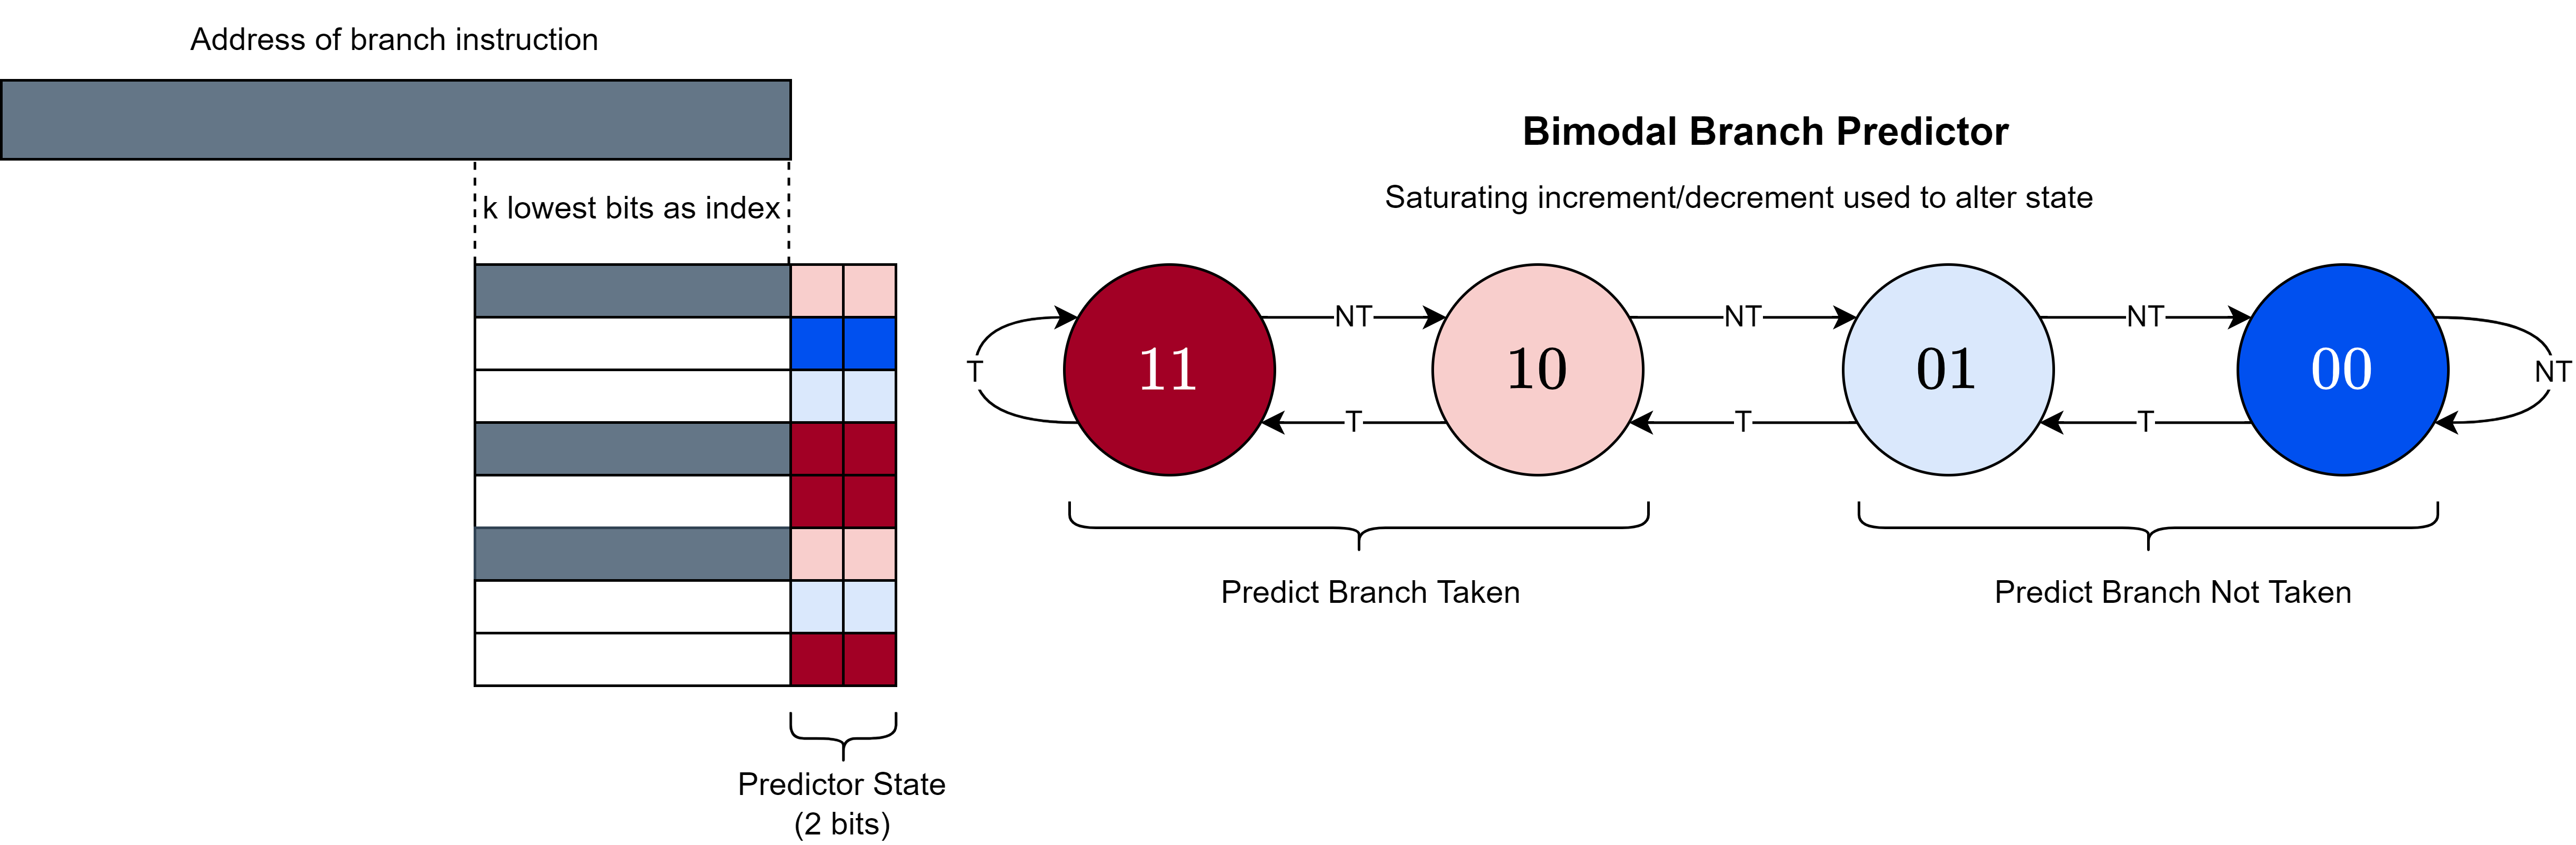
\includegraphics[width=.9\textwidth]{modelling/images/bimodal.drawio.png}
\end{center}
Hence we can also model the branch predictor state as a \textit{markov chain}.
\begin{definitionbox}{Stationary Diustribution}
    A probability distribution for a specific \textit{markov chain} that remains the same (stationary) as time progresses.
    \\
    \\ Given the transition matrix $\mathbf{P}$ of a chain, the stationary distribution can be represented by a vector of probabilities for being in any given state $\pi_\infty$ such that:
    \[\mathbf{P} \pi_\infty = \pi_\infty\]
    Hence $\pi_\infty$ is an eigenvector of $\mathbf{P}$ with associated eigenvalue $1$.
    \begin{itemize}
        \item It describes the probability of being in each state after infinite steps. 
    \end{itemize}
\end{definitionbox}
\begin{center}
    \begin{tabular}{r c | c c}
        & & \multicolumn{2}{c}{Actual Takeness} \\
        & & \textbf{Taken} & \textbf{Not Taken} \\
        \hline
        \multirow{2}{*}{Prediction} & \textbf{Taken} & Correct & Mispredict\\
        & \textbf{Not Taken} & Mispredict & Correct \\
    \end{tabular}
\end{center}
\[P(\text{Mispredict}) = P(\text{Predict Taken}) \times P(\text{Actually Not Taken}) + P(\text{Predict Not Taken}) \times P(\text{Actually Taken}) \]


\section{Modelling an Entire System}
Modelling an entire system is typically infeasible (scale and noise). Instead specific components and paths can be modelled.
\begin{enumerate}
    \item Identify code that matters for performance using a profiler (Hot code sections, called bottlenecks in vtune)
    \item Re-create behaviour in a controlled environment (\textit{microbenchmarking})
    \item Create an analytical model of the code path/component. 
    \item Validate the model with experimental results.
\end{enumerate}

